\chapter{Functions}
\label{chfuns}

\section{Functions}

Functions are arguably at the heart of mathematics and are the most
important definition of the whole course.

\begin{defn}
A \defini{function} $f\colon A\to B$ (for two sets $A$ and $B$) is a relation $R\subset
A\times B$ with the properties that
\begin{enumerate}
\item 
For every $a\in A$ there is a pair $(a,b)\in\R$: The domain of $R$ equals the source $A$.
\item
There
are no two pairs $(a,b),(a,c)\in R$ that share the same first entry.
(Formally: 
For all $a\in A$ and $b,c\in B$, if $(a,b)\in R$ and
$(a,c)\in R$, then $b=c$.)
\end{enumerate}
If this is the case, we can interpret the relation entry $(a,b)\in R$ (which
will be the only one for a given $a$) as {\em assigning} the \defini{value}
$f(a)=b$ to the \defini{argument} $a$. As with relations, we call 
\[
I=\{b\in B\mid \exists a\in A: (a,b)\in R\}
\]
the \defini{range} or \defini{image} of $f$.
See \figuref{figgeneralfct} for illustration.
\end{defn}

\begin{figure}[t]
\begin{center}
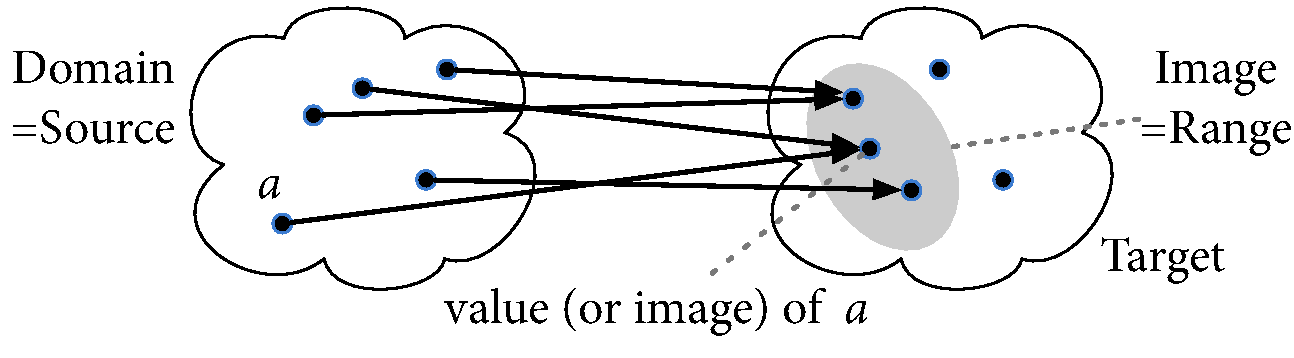
\includegraphics[width=6cm]{pic/GeneralFct.pdf}
\end{center}
\caption{A function}
\label{figgeneralfct}
\end{figure}

In short, a function is a rule that assigns for every element of its domain 
a unique element of its range.

Sometimes the term \defini{map} or \defini{mapping} is used synonymously
with {\em function}.

For relations on $\Q$ or $\R$ (or subsets thereof), the condition of being a
function can be
visualized in the graph if the relation by the property that no two points
of the relation lie on a vertical line. In the examples in
\figuref{figsomeRelations}, only the relation b) is a function, the others
are not.
\smallskip

What is important is to distinguish function $f$ (though sometimes we will write $f(x)$
to denote the function), argument $a$, and value
$f(a)$ of an
argument as three different (but related) entities. The argument is an
input, the function a machine (or an algorithm), and the value the output.
\smallskip

Two functions are equal if they have the same domain, the same target, and
(and this is the most important property)
if they assign to every element of the domain the same value.
%\method{Equality of functions}
To show that two functions $f,g$ are equal, we need to compare their
domains, their codomains, and finally show that for \textbf{every} $x$ in the
domain we have that $f(x)=g(x)$.
But if $f(a)=g(a)$ for just one argument $a$, this does not imply equality
of the functions.

Thus the function $f\colon\Z\to\Z$, that maps every $x\in Z$ to $(-1)^x$ is
equal to the function $g\colon\Z\to\Z$ that maps $x\in Z$ to $1$, if $x$ is
even, and to $-1$ otherwise. The functions are equal, since they give the
same values, even though the mechanism how they do so is different.

\subsection{Describing Functions}
Since functions are relations, they can be specified by
text, formula, table, distinction, picture,
to name just a few ways. 

In most cases, the easiest way of describing a function is by
using the interpretation of assigning values to elements of
their domain. That is, we specify
its domain, its target, and a rule (this can be a formula, or an algorithm)
that specifies the value of the
function for every element of the domain. This value must be an element of
the target.

Concretely, we write the name of the
function, a colon $\colon$, the domain, an arrow, and the codomain. If the
value is given by a formula, often the notation $a\mapsto f(a)=\mbox{formula}(a)$
is used. In many cases, it is convenient to describe a function informally
by text and makes for easier understanding. On the other hand, a formal
description avoids ambiguity and often makes it easier to formally prove
statements. Finally formal definitions are often easier to implement of a
computer.

The following thus are all perfectly good definitions of functions:
\begin{enumerate}
\item  Let $A=\{\mbox{frog},\mbox{horse},\mbox{sheep}\}$ and $B$ the set of
colors. We define $f_1\colon A\to B$ by assigning to each animal its outer
color:
\[
f_1\colon \left\{\begin{array}{lcl}
\mbox{frog}&\to&\mbox{green}\\
\mbox{horse}&\to&\mbox{brown}\\
\mbox{sheep}&\to&\mbox{black}\\
\end{array}
\right..
\]

\item Another function $f_2$ with same domain and target might assign to each animal its favorite color, say
\[
f_2\colon \left\{\begin{array}{lcl}
\mbox{frog}&\to&\mbox{green}\\
\mbox{horse}&\to&\mbox{red}\\
\mbox{sheep}&\to&\mbox{blue}\\
\end{array}
\right..
\]
This same function $f_2$ could be specified as
\[
f_2\colon a\to\left\{\begin{array}{ll}
\mbox{green}&\mbox{if $a=$frog,}\\
\mbox{red}&\mbox{if $a=$horse,}\\
\mbox{blue}&\mbox{if $a=$sheep.}\\
\end{array}
\right.
\]
Or someone might draw the function pictorially, as in
\figuref{figfroghorsesheep}.
\begin{figure}[t]
\begin{center}
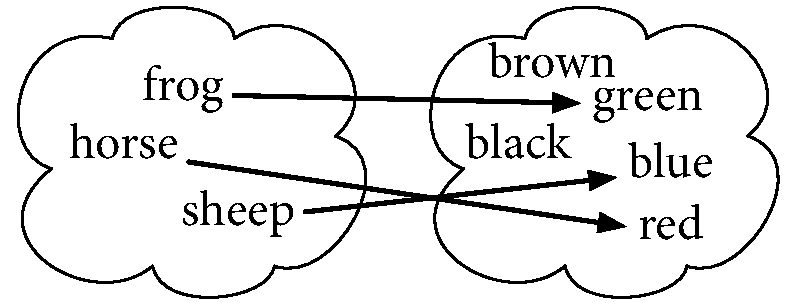
\includegraphics[width=6cm]{pic/AnimalColor.pdf}
\end{center}
\caption{A function assigning colors to animals}
\label{figfroghorsesheep}
\end{figure}

\item Let $A$ be the set of students at this university and $B$ the set of
symbol strings. The function $f_3\colon A\to B$ assigns to every student their
(preferred) first name. \label{fctex3}
\item Let $A,B$ as in example~\ref{fctex3}.
The function $f_4\colon A\to B$ assigns to each student
their email password. (It is a function, even though we cannot determine the
password used by a particular student.)
\item Let $D$ be the set of days of the current year and $T$ the set of
minutes in a day. We define the ``sunrise time in Denver'' function $f_5\colon
D\to T$ as assigning to each date the time of sunrise (in Denver, CO).
\item Let $S$ the set of students in this class and $G$ the set of grades.
Define $f_6\colon S\to G$ the function that assigns each student the
grade they will obtain in the class.
(To be a function, it is only required that the value is unique and
unambiguous, not that it is easily computable or known at the moment)
\item For $A=\N$ the set of nonnegative integers,
let $f_7\colon A\to A$, $x\mapsto x+1$. Other examples would be
$f_8\colon A\to A$, $x\mapsto x$, or
$f_9\colon A\to A$, assigning to $x$ the number of digits $x$ requires in
decimal representation.\mynote{You might note that we could alternatively
write $f_9(x)=\lfloor\log_{10}(x)\rfloor+1$, using the $\lfloor\cdot\rfloor$
notation for truncation.}
\item Let $f_{10}\colon \R\to\R$, $x\mapsto\frac{x^3+x+1}{x^2+1}$.
\item Left $f_{11}\colon\R\to\R$, $x\mapsto\begin{cases}
1&x<0\\
-2&x=0\\
x+17&0<x<1\\
\cos(x)&x\ge 1\\
\end{cases}$.
\item Let $g\colon\N\to\Q$ to give for each $n$ the first $n$ decimal
places of $\pi$. Thus $g(0)=3$, $g(1)=3.1$, $g(2)=3.14$ and so on. If we go
back to the notation of relations, we get
\begin{eqnarray*}
g&=&\{(n,\mbox{$\pi$ to $n$ decimal digits}\}\\
&=&\{(0,3),(1,3.1),(2,3.14),(3,3.141),(4,3.1415),\ldots\}.
\end{eqnarray*}
\end{enumerate}

On the other hand, the following attempts do not define functions (for
reasons indicated).
\begin{enumerate}
\item The relation $R=\{(a^2,a)\mid a\in\Q\}\subset\Q\times\Q\}$ is not a
function, {\em since there are multiple elements in $R$ -- e.g. $(4,2)$ and
$(-4,2)$ with the same first entry, so images are not uniquely defined.}
\item
Let $f\colon\Q\to\Z$ assigning to every rational number the
closest integer. {\em Not a function, as the closest integer is ambiguous,
say for $1/2$.} We can fix it, by defining an explicit tie-break rule for
ambiguous cases. (What is often used in practice is to take the largest integer $\le
x+\frac{1}{2}$.)
\item
Let $f\colon\Q\to\Q$, $x\mapsto\frac{x^2-1}{x-1}$. {\em This is not a function,
as the denominator at $x=1$ becomes zero.} One could fix it by changing the
domain to $\Q\setminus\{1\}$, or by replacing it with the function $x\mapsto
x+1$ (which for all $x\not=1$ returns the same value).
\item
Let $f\colon\Q\to\Q$, $x\mapsto\sqrt{x}$. {\em Not a function, as values,
such as $\sqrt{2}$ are not rational, and for negative $x$ are not defined in $\Q$.}
We can fix this by changing the domain to $\Q_{\ge 0}=\{a\in\Q\mid
a\ge 0\}$ and the target to $\R$.
\item Assigning to every subset of the rational numbers its smallest
element. {\em Not a function, since e.g. the set $\{a\in\Q\mid a>0\}$ has no
smallest element.} (We could fix this using the concept of
limits\pointer{seclimits}.)
\end{enumerate}

\section{Some Basic Functions}

It will be helpful to have a number of examples of functions at hand:
\medskip

First, take a set $A$ and let $B=A$. The \defini{identity function} on $A$ is
$\mbox{id}\colon A\to A$, $a\mapsto a$ the function that maps every element to the same
image.

\medskip
Let $A,B$ be sets and $b\in B$ some element. The \defini{constant function} (with value
$b$) is the function $A\to B$, $a\mapsto b$. If $A=B=\R$, the graph of the constant
function is a horizontal line.

\medskip

Let $A$ be a set and $S\subset A$. We let $B=\{0,1\}\subset \Q$. The
\defini{characteristic function} for $S$ is
\[
\chi_S\colon A\to B, a\mapsto\left\{\begin{array}{cl}
1&\mbox{if $x\in S$}\\
0&\mbox{if $x\not\in S$}\\
\end{array}
\right.
\]
A use of such a function is to ``crop'' another function, by multiplying with $\chi_S$,
for the product to be zero outside $S$.

\subsection{Polynomials and Rational Functions}

Many interesting function on numbers (i.e. $A\subset\R$) are given by
prescribing the image of $x\in A$ by a formula. The easiest version are
formulas that only involve addition and multiplication (including powers of
$x$). Such a function is called a polynomial function.

For example $f\colon\Q\to\Q$, $x\mapsto x^5-3x^2+17x+3$ is such a function.
The highest power of $x$ that arises (in the example: $5$) is called the
\defini{degree} of the polynomial, and the factors in front of powers of $x$
are called \defini{coefficients} of the polynomial.
We can describe the general case of a polynomial as
\[
c_d\cdot x^d+c_{d-1}x^{d-1}+\cdots+c_2x^2+c_1x+c_0=\sum_{i=0}^d c_ix^i
\]
where the $c_i\in\Q$ are the coefficients.
\bigskip

If $f$ and $g$ are both polynomials, and $A\subset\R$ such that $g(a)\not=0$
for all $a\in A$, we can also take the quotient $f(x)/g(x)$ as a new
function. It is called a \defini{rational function}.

\section{Function Arithmetic and Shifts}
\label{secfunari}

\begin{figure}
\begin{center}
\begin{tabular}{lll}
\begin{minipage}[t]{3.5cm}
a) $f(x)=x^3-3x^2+2$\\
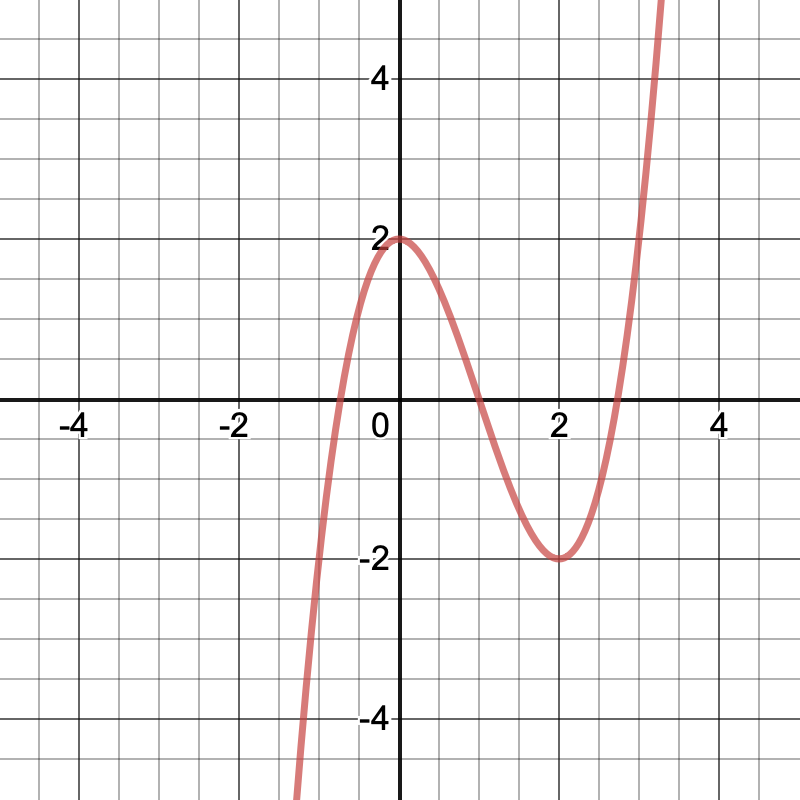
\includegraphics[width=3cm]{pic/fctshift0.png}
\end{minipage}&\begin{minipage}[t]{3.5cm}
b) $f(x)+1$\\
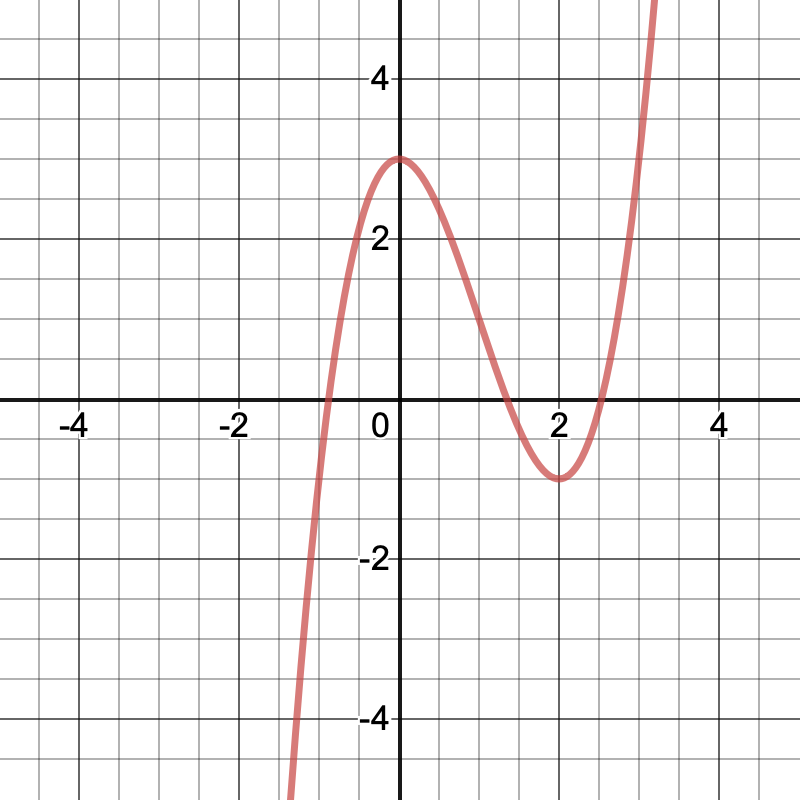
\includegraphics[width=3cm]{pic/fctshift1.png}
\end{minipage}&\begin{minipage}[t]{3.5cm}
c) $f(x)-3$\\
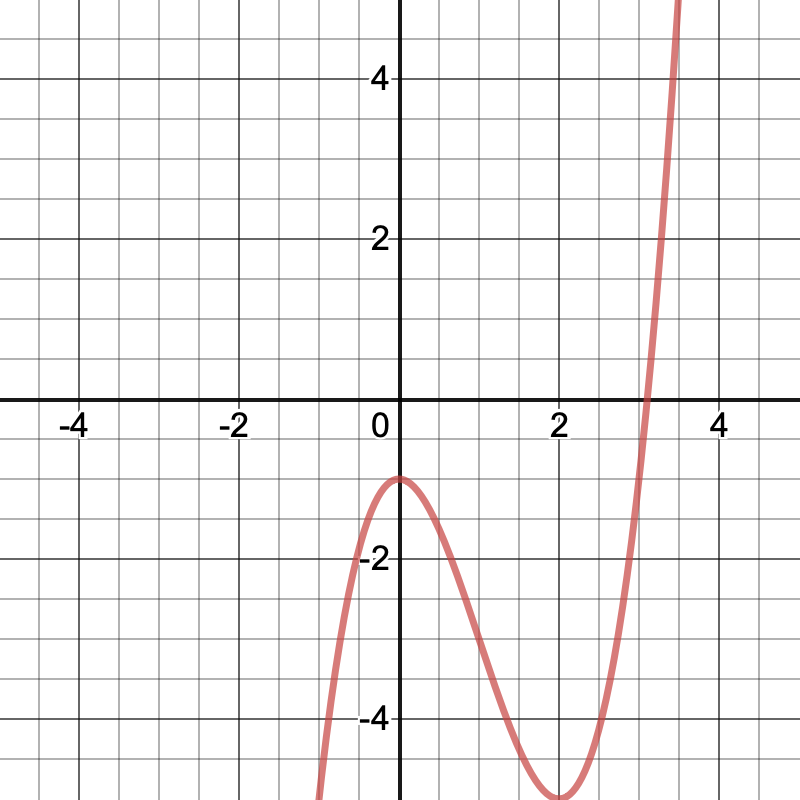
\includegraphics[width=3cm]{pic/fctshift2.png}
\end{minipage}\\
\\
\begin{minipage}[t]{3.5cm}
d) $-f(x)$\\
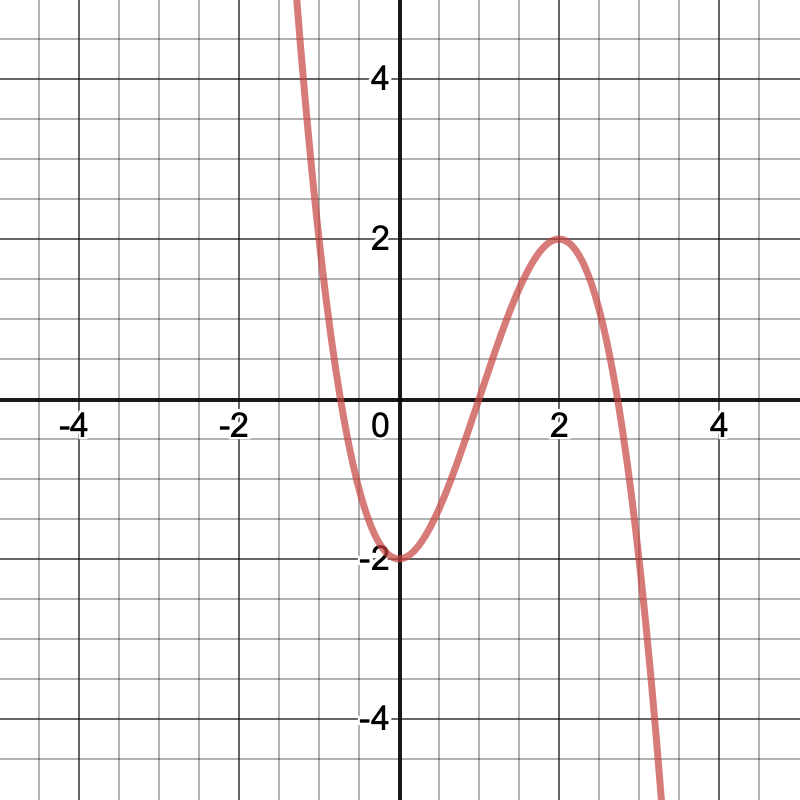
\includegraphics[width=3cm]{pic/fctshift3.png}
\end{minipage}&\begin{minipage}[t]{3.5cm}
e) $2-f(x)$\\
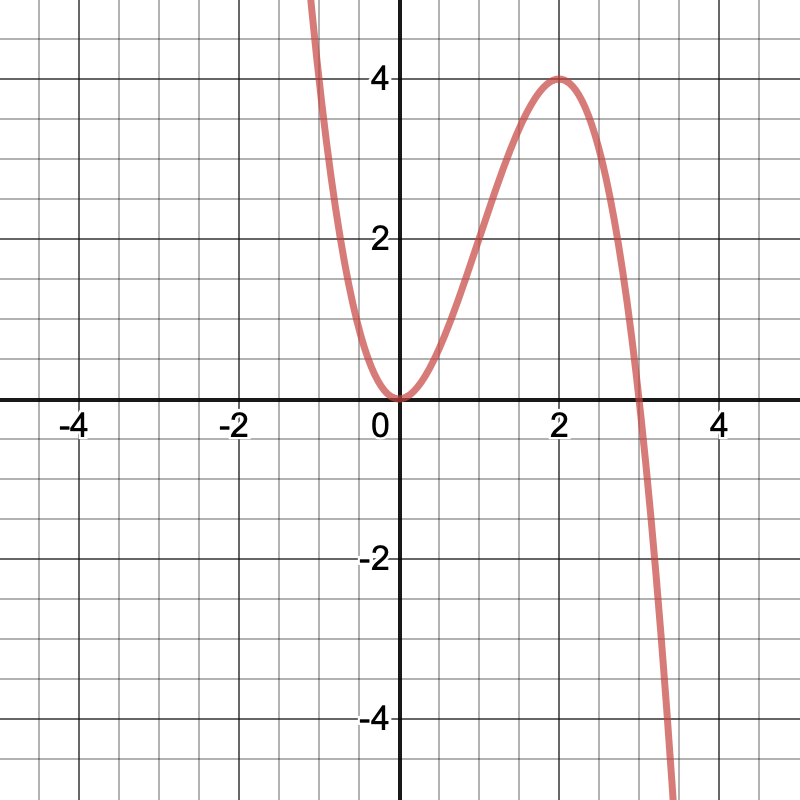
\includegraphics[width=3cm]{pic/fctshift4.png}
\end{minipage}&\begin{minipage}[t]{3.5cm}
f) $2f(x)$\\
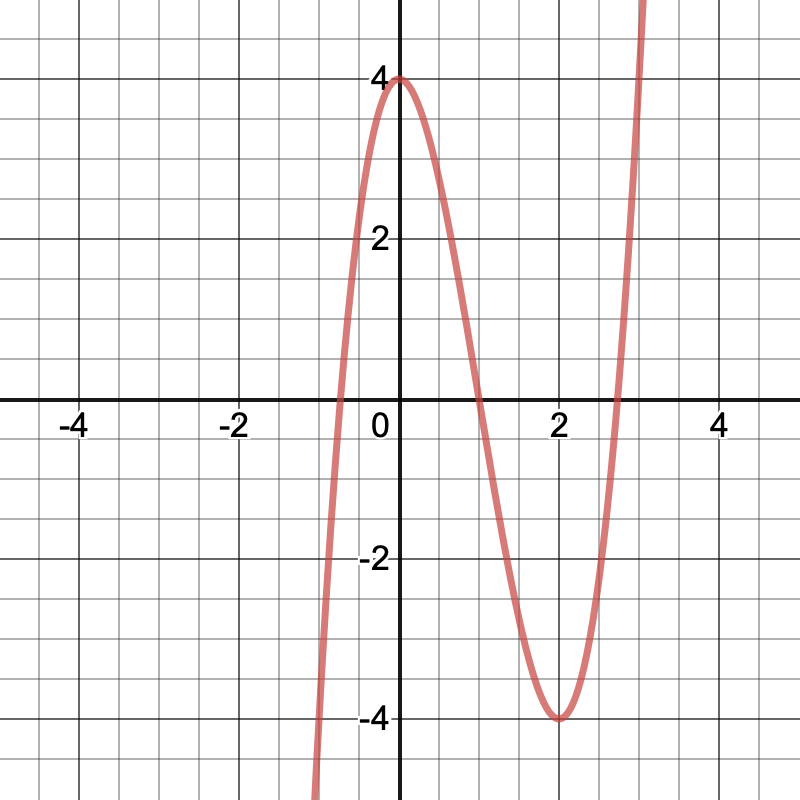
\includegraphics[width=3cm]{pic/fctshift10.png}
\end{minipage}\\
\\
\begin{minipage}[t]{3.5cm}
g)$-1/3\cdot f(x)$\\
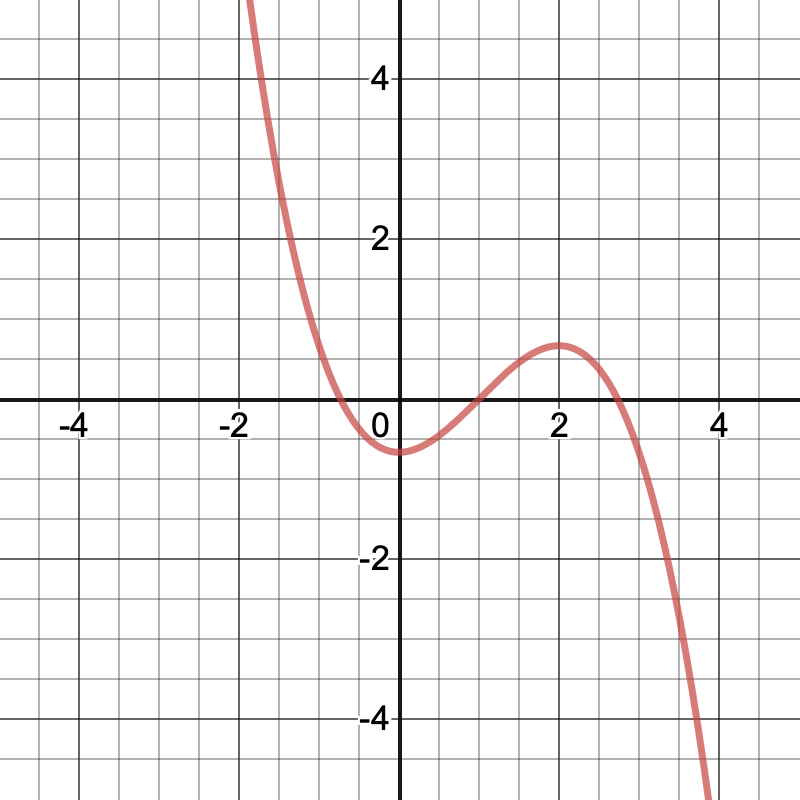
\includegraphics[width=3cm]{pic/fctshift11.png}
\end{minipage}&\begin{minipage}[t]{3.5cm}
h) Sum of $f(x)$ and $x^2$\\
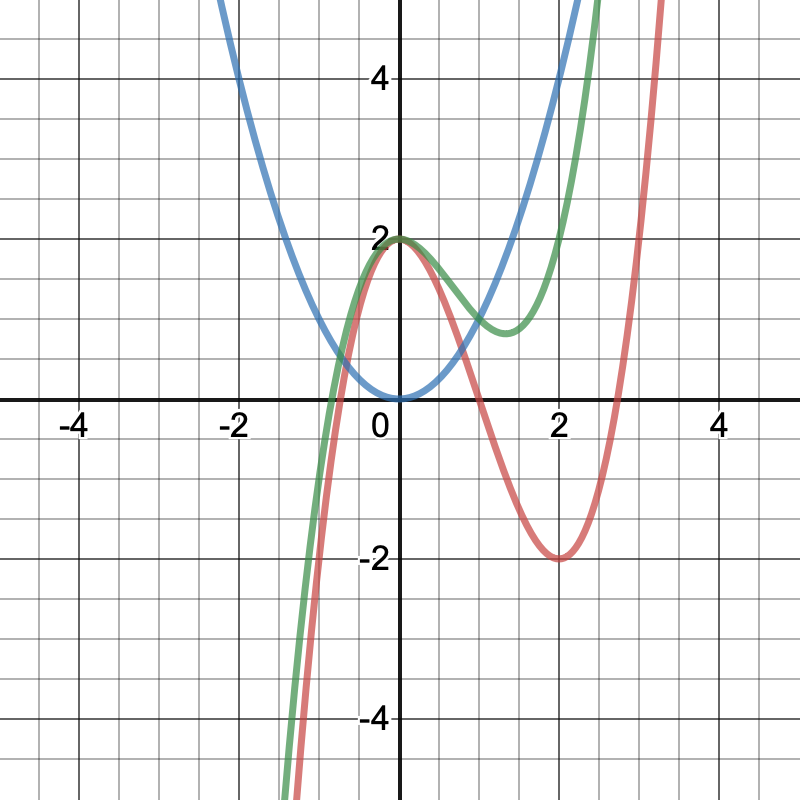
\includegraphics[width=3cm]{pic/fctshift9.png}
\end{minipage}&\begin{minipage}[t]{3.5cm}
i) $f(x+2)$\\
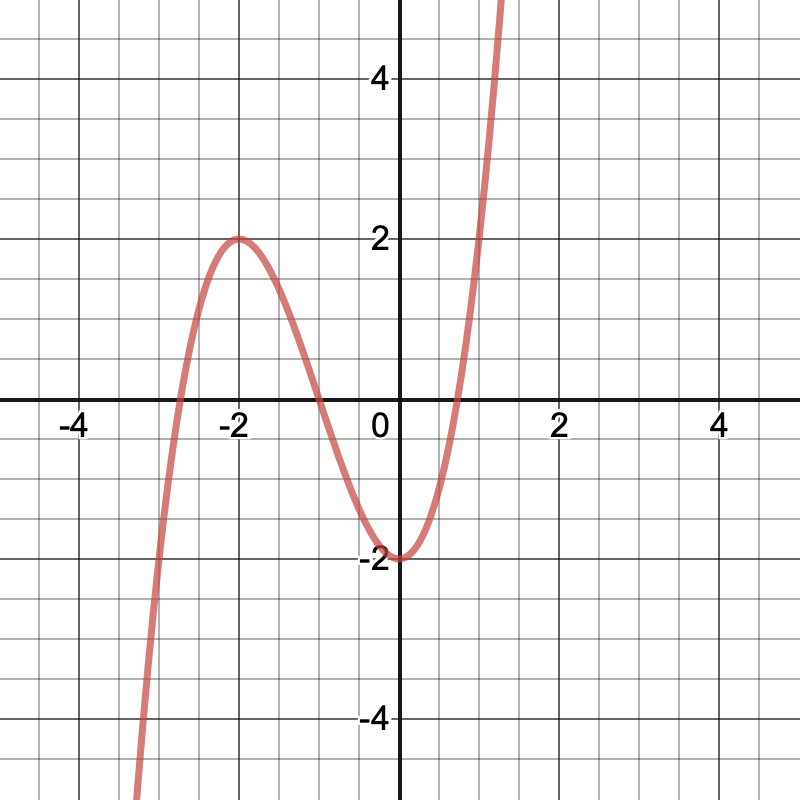
\includegraphics[width=3cm]{pic/fctshift6.png}
\end{minipage}\\
\begin{minipage}[t]{3.5cm}
j)$f(x-1)$\\
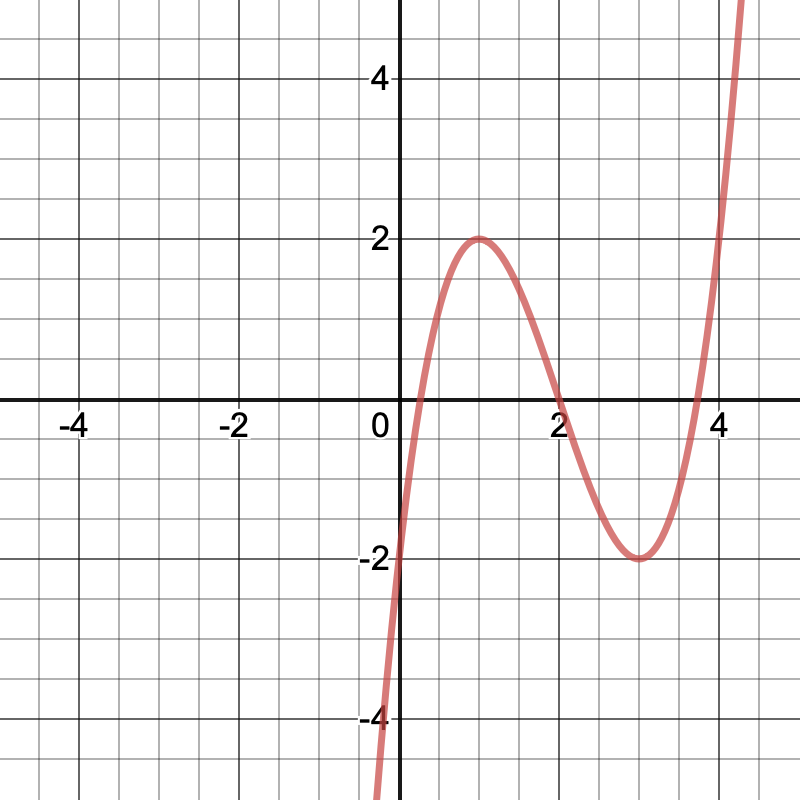
\includegraphics[width=3cm]{pic/fctshift5.png}
\end{minipage}&\begin{minipage}[t]{3.5cm}
k) $f(\frac{2}{3}x)$\\
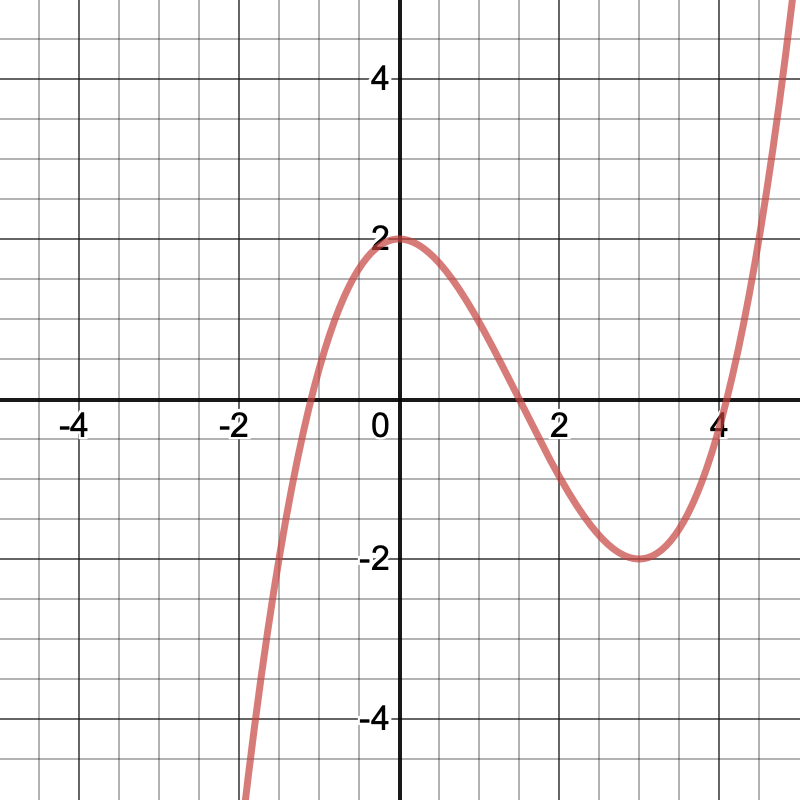
\includegraphics[width=3cm]{pic/fctshift12.png}
\end{minipage}&\begin{minipage}[t]{3.5cm}
l) $f(-\frac{3}{2}x)$\\
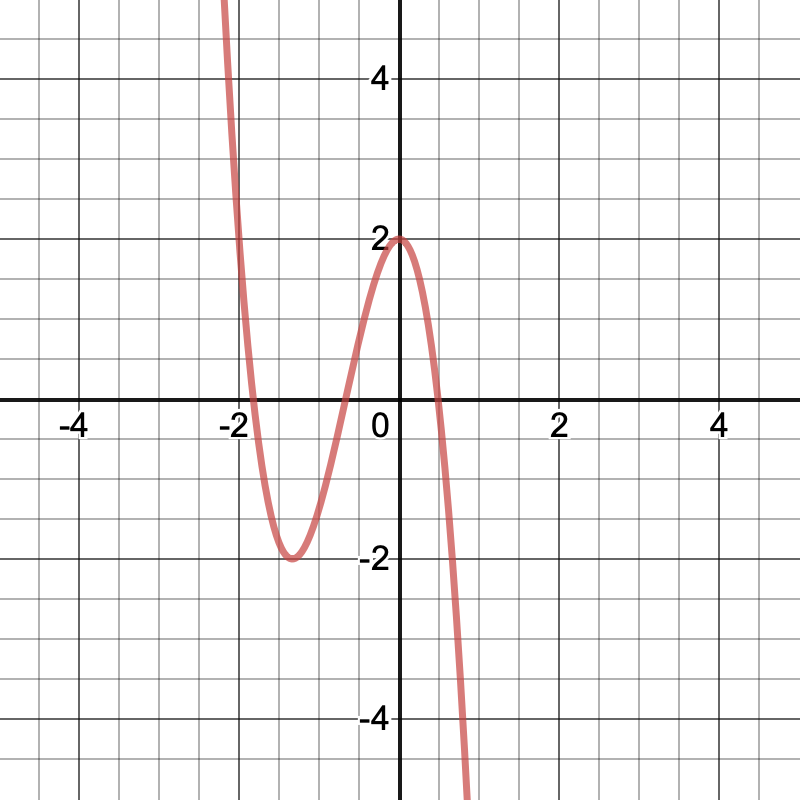
\includegraphics[width=3cm]{pic/fctshift13.png}
\end{minipage}\\
\end{tabular}
\end{center}
\caption{Transformations of a function}
\label{figfctTrafo}
\end{figure}

We want to investigate what happens how a function (and the graph of a
function) under arithmetic operations. This also can be useful to modify a
given function in a desired way.

We illustrate this, using an example (Figure~\ref{figfctTrafo}, we transform the
function given under a)): If we add a constant to $f$, i.e. replace $f(x)$ by $f(x)+k$
we add $k$ to all function values. This means the graph of $f$ shifts up by $k$ units
(b), respectively down (c) if $k$ is negative.

If instead we subtract $f$ from a constant (d) and e)) we get the graph of $f$, flipped
upside down and shifted vertically.

Multiplying by a constant will stretch (f) the graph vertically by this factor, respectively
compress if the factor is (of absolute value) $<1$ and flip if negative (g).
\smallskip

More generally, we can take the sum of two functions, which is the function $f+g$ that
assigns to each $x$ the value $f(x)+g(x)$. See figure h) for $g(x)=x^2$ in blue and
$f(x)+x^2$ in green.
\medskip

So far, all transformations were vertical. To transform horizontally, we need to modify
the argument $x$ instead of the value $f(x)$:
First consider if we replace $x$ by $x+k$. Then $f(x+k)$ assigns to a point $a$ the
value $f(a+k)$ that $f$ has at $a+k$, that is $k$ units {\em to the right} of $a$.
The effect is to shift the
graph {\em to the left} by $k$ units (i) for positive $k$, respectively to the right for
negative $k$ (j).
Similarly, multiplying $x$ by a factor $k$ will assign to $a$ the value $f(k\cdot a)$
that $f$ has at $k$ times $a$. Thus for $0<\sz{k}<1$ the graph will be stretched
horizontally (k), for $\sz{k}>1$ it will be compressed horizontally. And a negative $k$
flips left and right (l).
\medskip

In summary, adding to $f(x)$ or multiplying by a number will transform the graph
vertically as one would expect. Changing the argument transforms the graph horizontally,
but {\em in reverse} of what the same transformation would do vertically.

\subsection{Composition}
\label{secfunccomposition}

When, in the last section, we modified the argument $x$ of a function $f$ we actually
used a special case of the composition of function, composing $f$ with a function
$x\mapsto x+k$ or $x\mapsto kx$.

Since functions are relations, the composition of functions is just a special case of
the composition of relations. Suppose $f\colon A\to B$ and $g\colon B\to C$ are
functions. Then, as relations, we have that 
\[
f=\{(x,f(x)\mid x\in A\}
\qquad\mbox{and}\qquad
g=\{(y,g(y)\mid y\in B\}.
\]
By the definition of composition of relations, we thus get the composition $g\circ
f\subset A\times C$ as
\begin{eqnarray*}
g\circ f&=&\{(a,c)\mid \exists b\in B:(a,b)\in f \mbox{\ and\ }(b,c)\in g\}\\
&=&\{(a,c)\mid (b,c)\in g \mbox{\ for\ }(a,b)\in f\}\\
&=&\{(a,c)\mid c=g(b) \mbox{\ for\ }b=f(a)\}\\
&=&\{(a,g(f(a)))\mid a\in A\}.
\end{eqnarray*}
This means that $g\circ f$ is again a function (exercise: verify this) from
$A$ to $C$, mapping $x\mapsto g(f(x))$. This is also the justification for the notation
$g\circ f$, as we have that $(g\circ f)(x)=g(f(x))$.
\smallskip

Note that usually (even if $A=B=C$) $g\circ f\not=f\circ g$. For example, if
$f\colon\Q\to\Q$, $x\mapsto x+1$ and 
$g\colon\Q\to\Q$, $x\mapsto 2x$, then $g\circ f\colon x\mapsto 2(x+1)=2x+2$, while
$f\circ g\colon x\mapsto (2x)+1$.
\smallskip

Unless one of the function is relatively basic\mynote{these are \defini{linear}
functions}, that is only adding constants or multiplying with a scaling factor as we did
in the previous section, the effect of composition on the graph of the function is more
complicated than can be describe by easy rules.

\section{Properties of Functions}

When we looked at relations, we also had two other operations. Since functions are a
special case of relations, they also apply here, but are not always of interest: 
Taking the complement of a function will almost never be a function. We will study the
question of whether the converse of a function is a function (and not just a relation)
in this section.
\medskip

The definition of a function had two requirements. We will define two properties that a
function $f\colon A\to B$ might have. These properties correspond to the two requirements holding for the converse relation.

Fundamentally, the relation form of $f$ is $\{(a,f(a))\mid a\in A\}$ and the converse
thus is $\{(f(a),a)\mid a\in A\}$. We want to write this instead in
the form $\{(b,\mbox{something})\mid b\in B\}$. This means that testing for the properties
is related to solving $b=f(a)$ for $a$.

\subsection{Onto}

A function is onto, if it takes every possible value, that is if its image
equals its target.
For example, we could take a function that maps the visitors of a hotel to
the hotels guest rooms. This function is onto whenever the hotel is booked
out.

Formally:
\begin{defn}
A function $f\colon A\to B$ is called \defini{onto} (some books instead use the posher
term \defini{surjective}), if every element of $B$ is obtained as an image, that is for every $b\in B$ there is an $a\in A$ such that $f(a)=b$.
\end{defn}

\begin{figure}[t]
\begin{center}
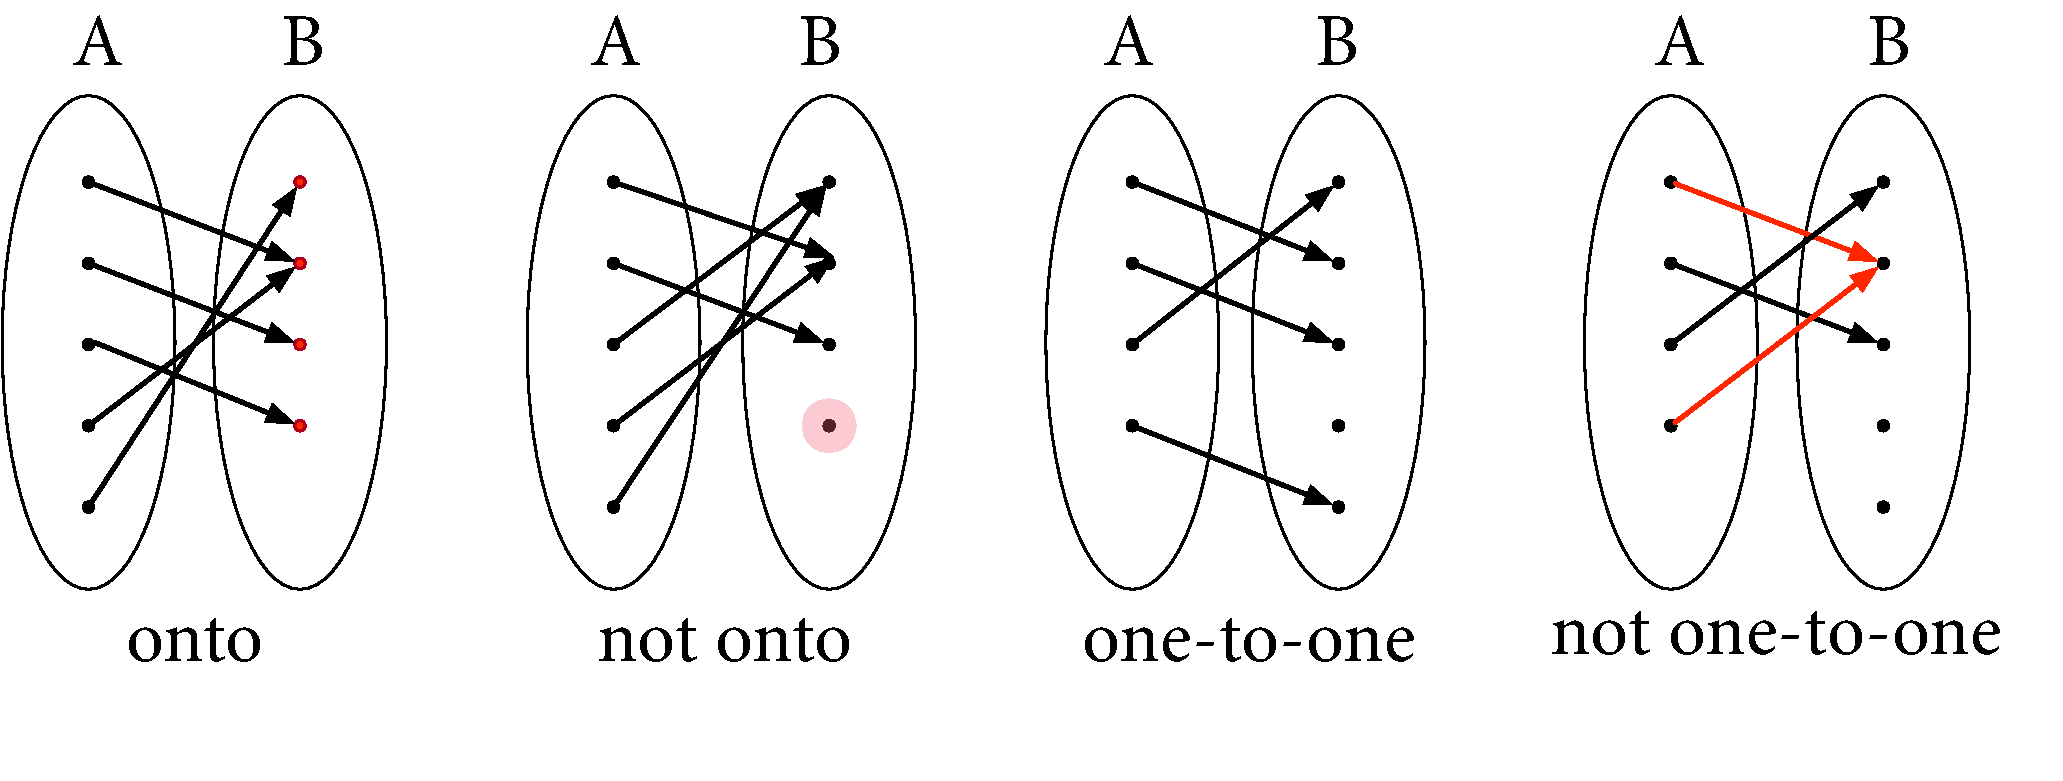
\includegraphics[width=\the\textwidth]{pic/OntoPics.pdf}
\caption{Onto and One-To-One}
\label{figoneonto}
\end{center}
\end{figure}

The left two images in Figure~\ref{figoneonto} illustrate the concept.

\begin{figure}[t]
\begin{center}
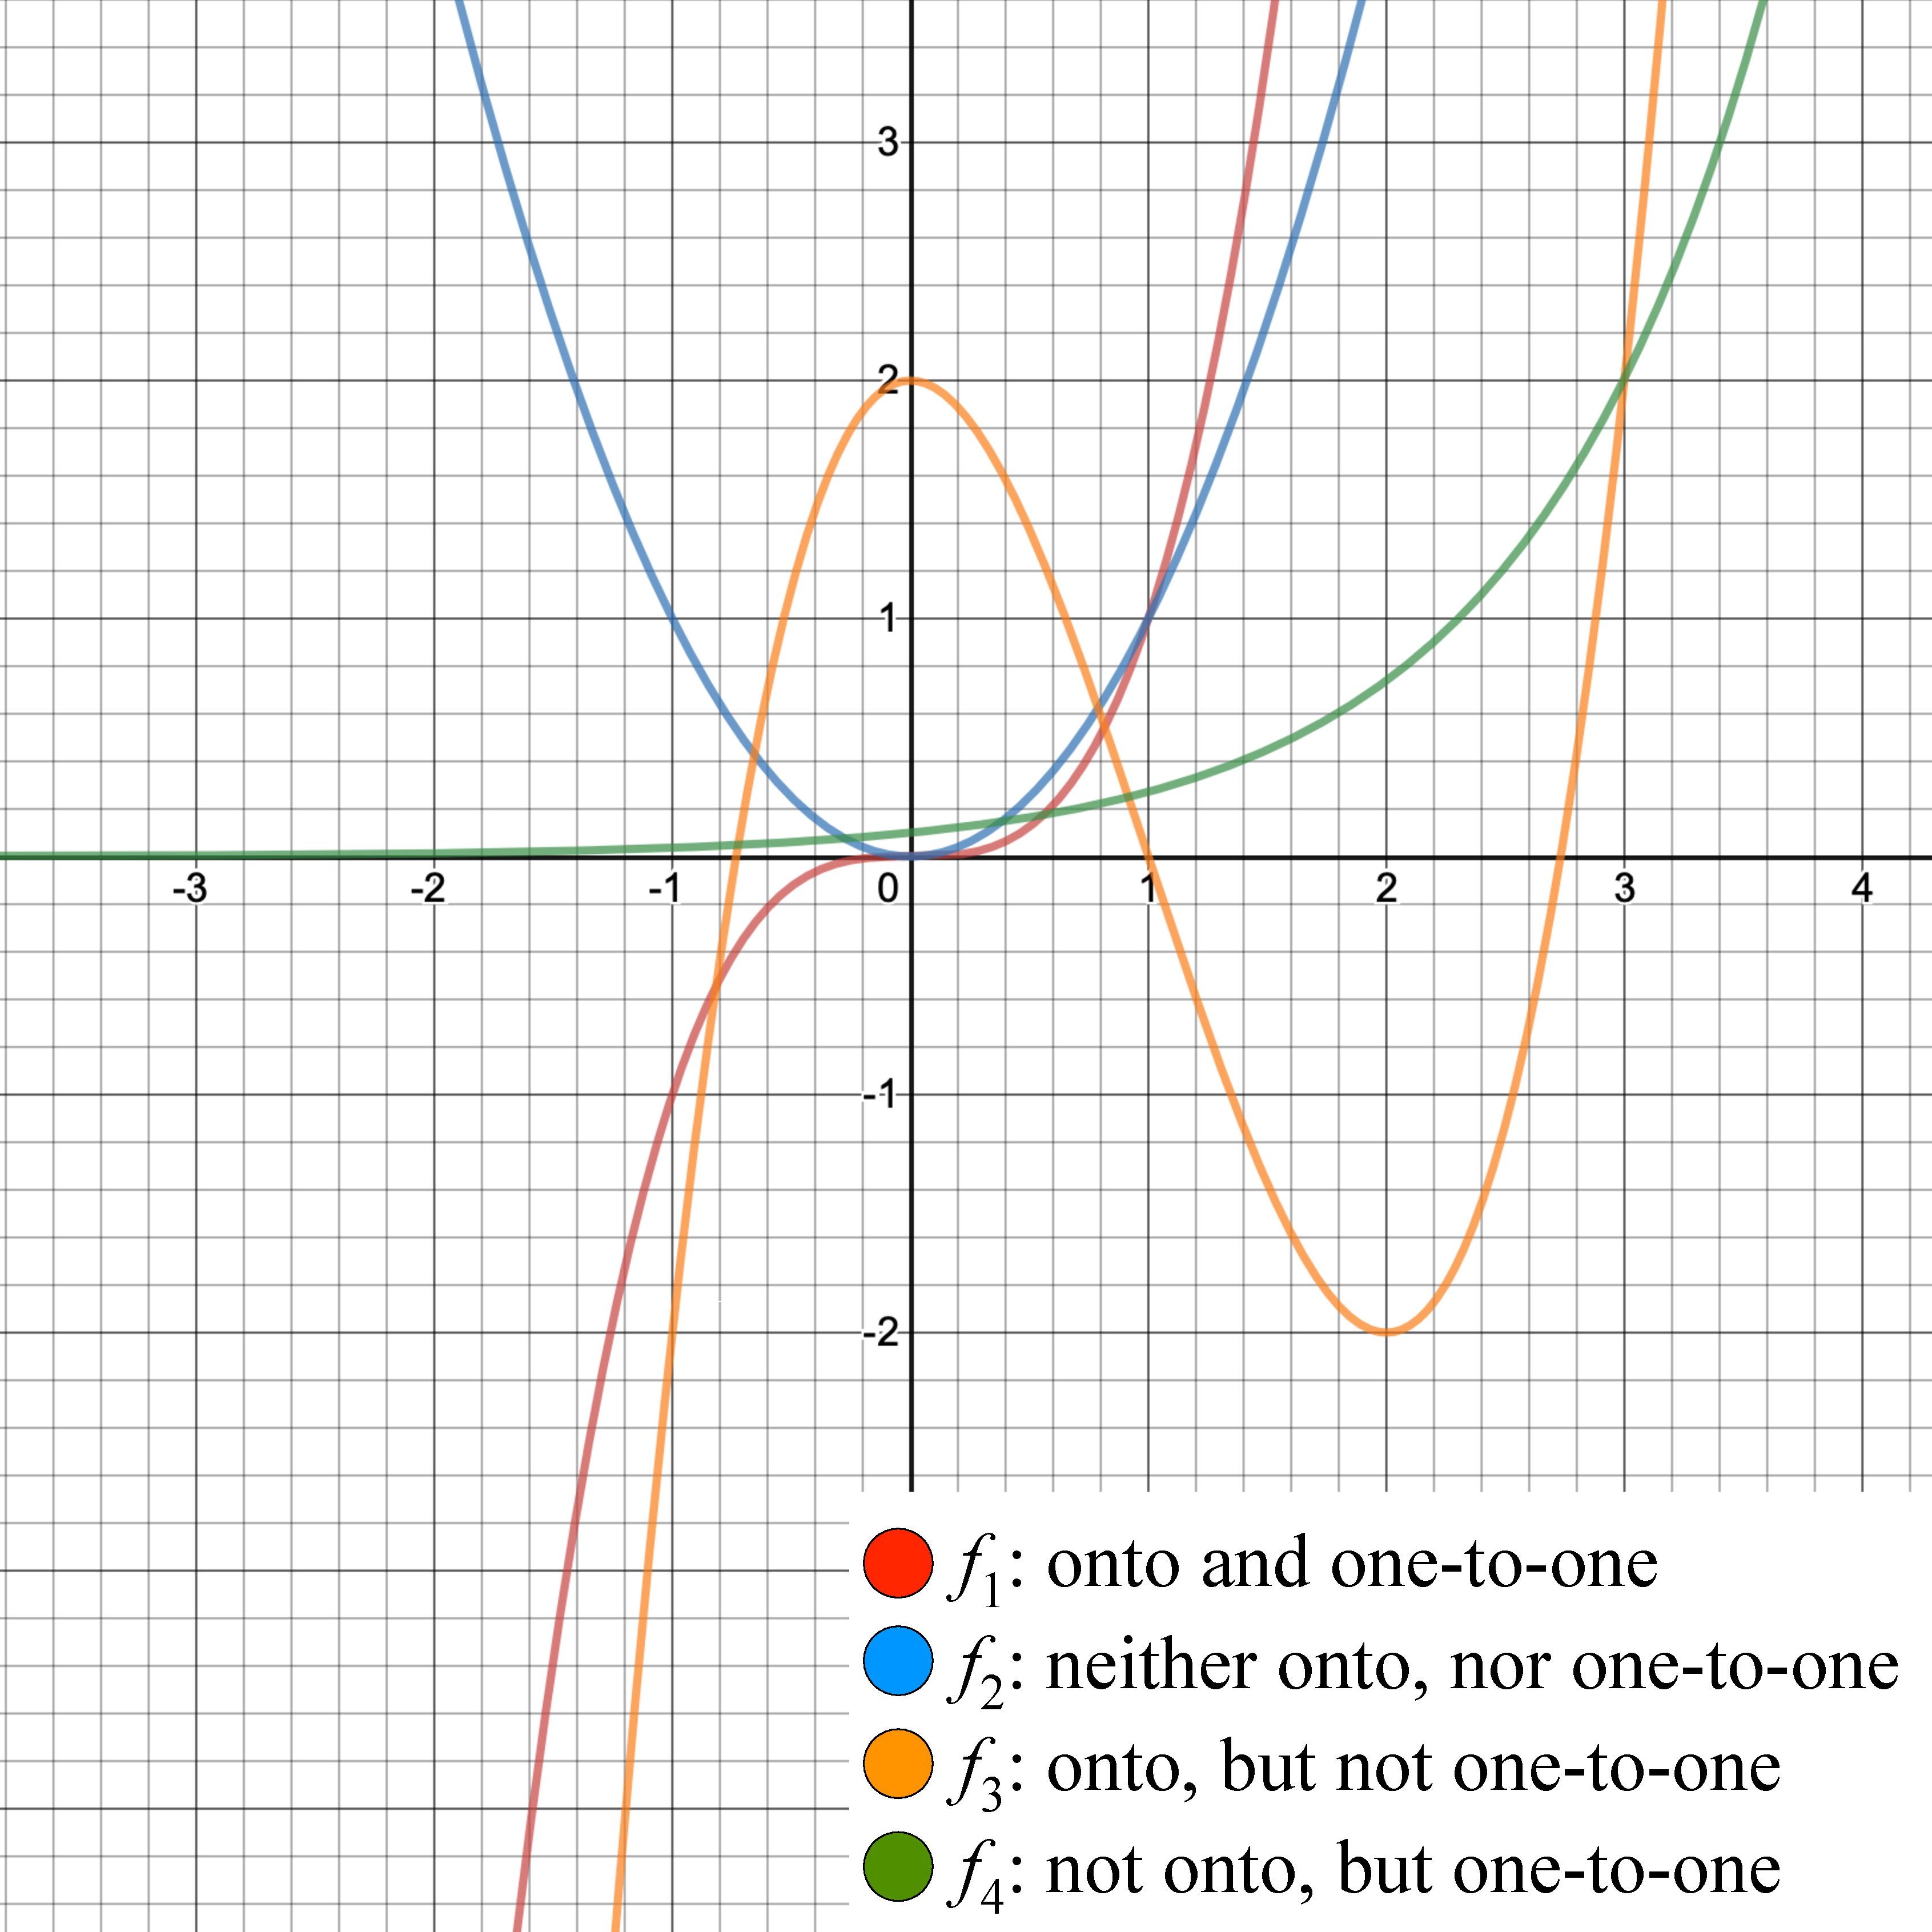
\includegraphics[width=8cm]{pic/OneToOneOnto.pdf}
\caption{Onto and One-To-One for functions $\R\to\R$}
\label{figoneontofcts}
\end{center}
\end{figure}

If a function is given by a graph, it is onto if the projection of the graph
on the $y$-axis is all of $B$, respectively that every horizontal line intersects the
graph.
For example (see Figure~\ref{figoneontofcts}), the function $f_1\colon\R\to\R$, $x\mapsto x^3$ is onto, while
the function $f_2\colon x\mapsto x^2$ is not onto (it takes only positive
values).

Similarly, $f_3\colon x\mapsto x^3-3x^2+2$ is
onto, but $f_4=\frac{1}{10}\exp(x)$ is not.

Note that the target defined for the function is crucial for a decision on
whether it is onto. If we change $f_2$ to a function $g_2\colon\R\to\R_{\ge
0}$, $x\mapsto x^2$ (i.e. same rule, just changed the target), then $g_2$ is
onto.
\medskip

To show algebraically that a function is onto, we need to show that every
element $b\in B$ in the target is obtained as image. The easiest way of
doing so is to find an explicit $a\in A$ such that $f(a)=b$. We might be
able to do so (but are not guaranteed) by solving for $a$.

For example, for function $f_1$ we have that $a=\sqrt[3]{b}$ is mapped to
$b$. On the other hand $f_3$ is also onto, but it is hard to solve for $a$,
and for $-2\le b\le 2$ there are multiple possible $a$.
\smallskip

A function being onto guarantees that the source of the converse relation
equals its domain, i.e. it has pairs
$(b,*)$ for every $b\in B$, 

\subsection{One-to-One}

In many situations of real-world functions $f\colon A\to B$, i.e. when
assigning objects in B to objects in A, the
intention is to use the assigned object in B in place of the original object in $A$.
That is, there is an assumption that for a given $b\in B$ we can look-up the unique
$a\in A$ for which $f(a)=b$. Examples of this are Social Security numbers, student ID
numbers, car number plates\footnote{That is the reason for a number plate such as
\texttt{COOLGUY14} -- the number 14 is not special, but 1--13 were used already},
or bar codes on supermarket items.

But this is not always guaranteed. If we map people to names, or dates of birth there
will be typically multiple matches, even in a limited population\mynote{This is of
course the reason why ID numbers were invented in the first place.}. It is thus an
interesting property, and in fact the one that ensures the second property for functions
for a converse.

\begin{defn}
A function $f\colon A\to B$ is called \defini{one-to-one} (some books instead use the posher
term \defini{injective}), if there are no two different elements $a_1,a_2\in A$,
$a_1\not=a_2$ such that $f(a_1)=f(a_2)$. In other words, if $f(a_1)=f(a_2)$ then
$a_1=a_2$.
\end{defn}

The right two images in Figure~\ref{figoneonto} illustrate the concept.
In the above example of mapping hotel visitors to bedrooms, the function is one-to-one
whenever every bedroom is single-occupancy (or empty).
\medskip

If a function is given by a graph, being one-to-one means that every {\em horizontal}
line intersects the graph in at most one point. Thus,
in the functions in Figure~\ref{figoneontofcts}, we have that $f_1$ and $f_4$ are
one-to-one, but the other two are not.

Again, being one-to-one does not only depend on the rule of the function, but its
declaration. It might be possible to restrict the domain $A$ to a subset $A_1\subset A$
and get a new function that is one-to-one. In the examples, both $f_2$ and $f_3$ would
become one-to-one, if we restricted their domain to $\{x\in\R|mid x>2\}$.
\medskip

To test algebraically for a function being one-to-one requires that one can solve
uniquely for $a$ with $f(a)=b$. This is for example the case for $f_1$ (as
$\sqrt[3]{b}$ is unique in the real numbers), but it is not true for $f_2$ (since
$f_2(-1)=f_2(1)$).

Doing so can be hard, we will see that calculus will provide better tools
for testing one-to-one~\pointer{secincr}.

An important application of the concept of one-to-one in computer science is
that of \defini{hash functions}. In short, a hash function takes a digital
object (stored information, or a binary file) and maps it to a large
integer. The hope is that the function is one-to-one\mynote{on the set of
plausible inputs. That is not all possible binary files, but say binary
files that would be valid programs. Often it is impossible to prove that
such a hash function is one-to-one, but the property is only observed
through examples or in approximation}, that is the hash value allows to
identify the data/file and for example to use the hash to verify that it has
not been tampered with but is the original file.

While a one-to-one function allows in principle to identify the original
argument $a$ from a function value $f(a)$ this may be hard (or impossible in
practice) to do for hash functions. Indeed part of the mechanism underlying
bitcoin and other digital currencies is that such a look-up seems to be hard
in practice and can only be done by trying out different values of $a$ and
checking when the desired value $f(a)$ is reached.
\medskip

We close with a connection between the concepts of onto and one-to-one in
the case of finite sets:
\begin{lemma}
\label{lemoneonto}
If $A$ and $B$ are finite sets with $\sz{A}=\sz{B}$, then a function $f\colon A\to B$ is
one-to-one, if and only it is onto.
\end{lemma}
\begin{proof}
We set $n=\sz{A}=\sz{B}$.
There are two directions to show. First assume that $f\colon A\to B$ is onto. If $f$ was
not one-to-one, there would be two different elements, $a_1,a_2\in A$, such that
$f(a_1)=f(a_2)$. But then $f$ would have to have strictly fewer than $n$ values in $B$
and thus could not be onto.\\
Vice versa, assume that $f\colon A\to B$ is one-to-one. If it was not onto, it would
have to have strictly fewer than $n$ values, which means that not all $n$ elements of
$A$ could have different images.
\end{proof}
Note that this lemma is false if the sets are infinite. The functions $f_3$ and $f_4$ in
Figure~\ref{figoneontofcts} are counterexamples.

\section{Bijections and Inverse Functions}

A function $f\colon A\to B$ that is both one-to-one and onto is called
\defini{bijective} or an \defini{bijection}. Being bijective means that for every $b\in
B$ there is a unique $a\in A$ such that $f(a)=b$.

The converse property, i.e. that for every
$a\in A$ there is a unique $b\in B$, is the definition of a function. This means that
the converse relation to $f$, namely
\[
\{(f(a),a)\mid a\in A\}
\]
is a function. We call it the inverse function to $f$, and call it $f^{-1}$. It is a
function $B\to A$ that maps $b$ to the unique $a$ such that $f(a)=b$.
Note that
this $\cdot^{-1}$ in the name is a pure formalism due to a limited set of symbols available. It
should \textbf{not} be confused with $1/f$, which is another function entirely\mynote{Formally, 
$1/f$ is the inverse under
pointwise multiplication $(f\cdot g)(x)=f(x)\cdot g(x)$, while $f^{-1}$ is the inverse
under composition of functions.}.
In the example of assigning people to hotel rooms, if the function is bijective, its the
inverse function assigns to a room its occupant.

By the definition, the relation form of the inverse function,
\[
\{(b,f^{-1}(b))\mid b\in B\},
\]
is the converse relation to $f$. We also
note that $f^{-1}\circ f\colon A\to A$, $a\mapsto f^{-1}(f(a))=a$ is the identity
on $A$, and that $f\circ f^{-1}\colon B\to B$, $b=f(a)\mapsto f(f^{-1}(b))=f(a)=b$ is
the identity on $B$.
\medskip

If $f$ is given by a formula for $f(a)$, one might be able to get a formula  from
solving $f(a)$ for $a$. For example, we have seen that the function $f_1\colon\R\to\R$,
$x\to x^3$ is onto and one-to-one, and its inverse will be the function
$f_1^{-1}\colon\R\to\R$, $x\mapsto\sqrt[3]{x}$. But the function $f_5\colon\R\to\R$,
$x\mapsto x^3+x$ is also one-to-one and  onto, but we will be hard pressed to solve
$a^3+a=b$ for $a$.

\section{Counting and Cardinality}
\label{defcardinality}

One use of bijective functions is how the cardinality of a set is actually defined.
Formally, we
define the cardinality of a set $A$ as the unique $n$, such that there is a bijective
function from $A$ to the set $\{1,2,\ldots,n\}$. (Formally, one has to show that this
$n$ will be always the same, regardless of the function chosen, but we will skip this
step here.) This function can be interpreted as numbering the elements when counting.

We give formulas for the cardinality of some of the set constructions. In the following,
let $A$ be a set with $\sz{A}=n$ and $B$ a set with $\sz{B}=m$:

\paragraph{Cartesian Product}
Once we numbered the elements of $A$ and $B$, we can consider the pairs in the Cartesian
product as coordinates in an $n\times m$ rectangle. Thus $\sz{A\times B}=n\cdot m$.

\paragraph{Power Set}
Every subset of $A$ can be described by bit-string of length $n$ that indicates for each
element of $A$ whether it is contained in the subset. These bit strings lie in the
$n$-fold Cartesian product $\{0,1\}\times\{0,1\}\times\cdots\times\{0,1\}$, and thus
there are $2^n$ such strings. Thus $\sz{{\cal P}(A)}=2^n$.

We note, without proof, that the number of subsets of fixed size $k$ is given by the
\defini{binomial coefficient}
\[
{n\choose k}=\frac{n!}{k!(n-k)!}
\]
(where $n!=1\cdot 2\cdot 3\cdot\cdots\cdot n$ is called $n$-\defini{factorial})

\paragraph{Relations}
Every relation is a subset of $A\times B$. Thus the number of relations between $A$ and
$B$ is $\sz{{\cal P}(A\times B)}=2^{n\cdot m}$.

\paragraph{Functions}
We can consider a function from $A$ to $B$ as an $n$-tuple that gives in position $i$
the value of the $i$-th element of $A$. The formula for the order of a Cartesian product
thus gives $\sz{B\times \cdots\times B}=m^n$ different functions.

\paragraph{One-to-One Functions}
To ensure the function is one-to-one, the image of the second element cannot be chosen
freely, but needs to be different than the image of the first element. Thus we do not
have $m$ choices, but only $m-1$ choices. And for the third element there are $m-2$
possible images and so on until the $n$-th element has $m-n+1$ possible images. Thus there are
\[
m\cdot (m-1)\cdot (m-2)\cdot \cdots\cdot (m-n+1)=m!/(m-n)!
\]
one-to-one functions. Note that this product has a factor $0$ (and thus becomes zero
itself) if $n>m$.

\paragraph{Bijective Functions}
Note that such functions can only exist if $n=m$, but then, by Lemma~\ref{lemoneonto},
it is sufficient for the function to be one-to-one. Thus there are $n!/(n-n)!=n!/1=n!$
bijective function if $m=n$ (and zero otherwise).

\paragraph{Onto Functions}
The formula for the number of onto functions is more complicated than could plausibly be
explained here. It is:
\[
\sum_{i=1}^m (-1)^{m-i}{m\choose i}i^n.
\]


